
\begin{figure}[t]
	\centering
		\begin{minipage}{0.225\textwidth}
			\centering
			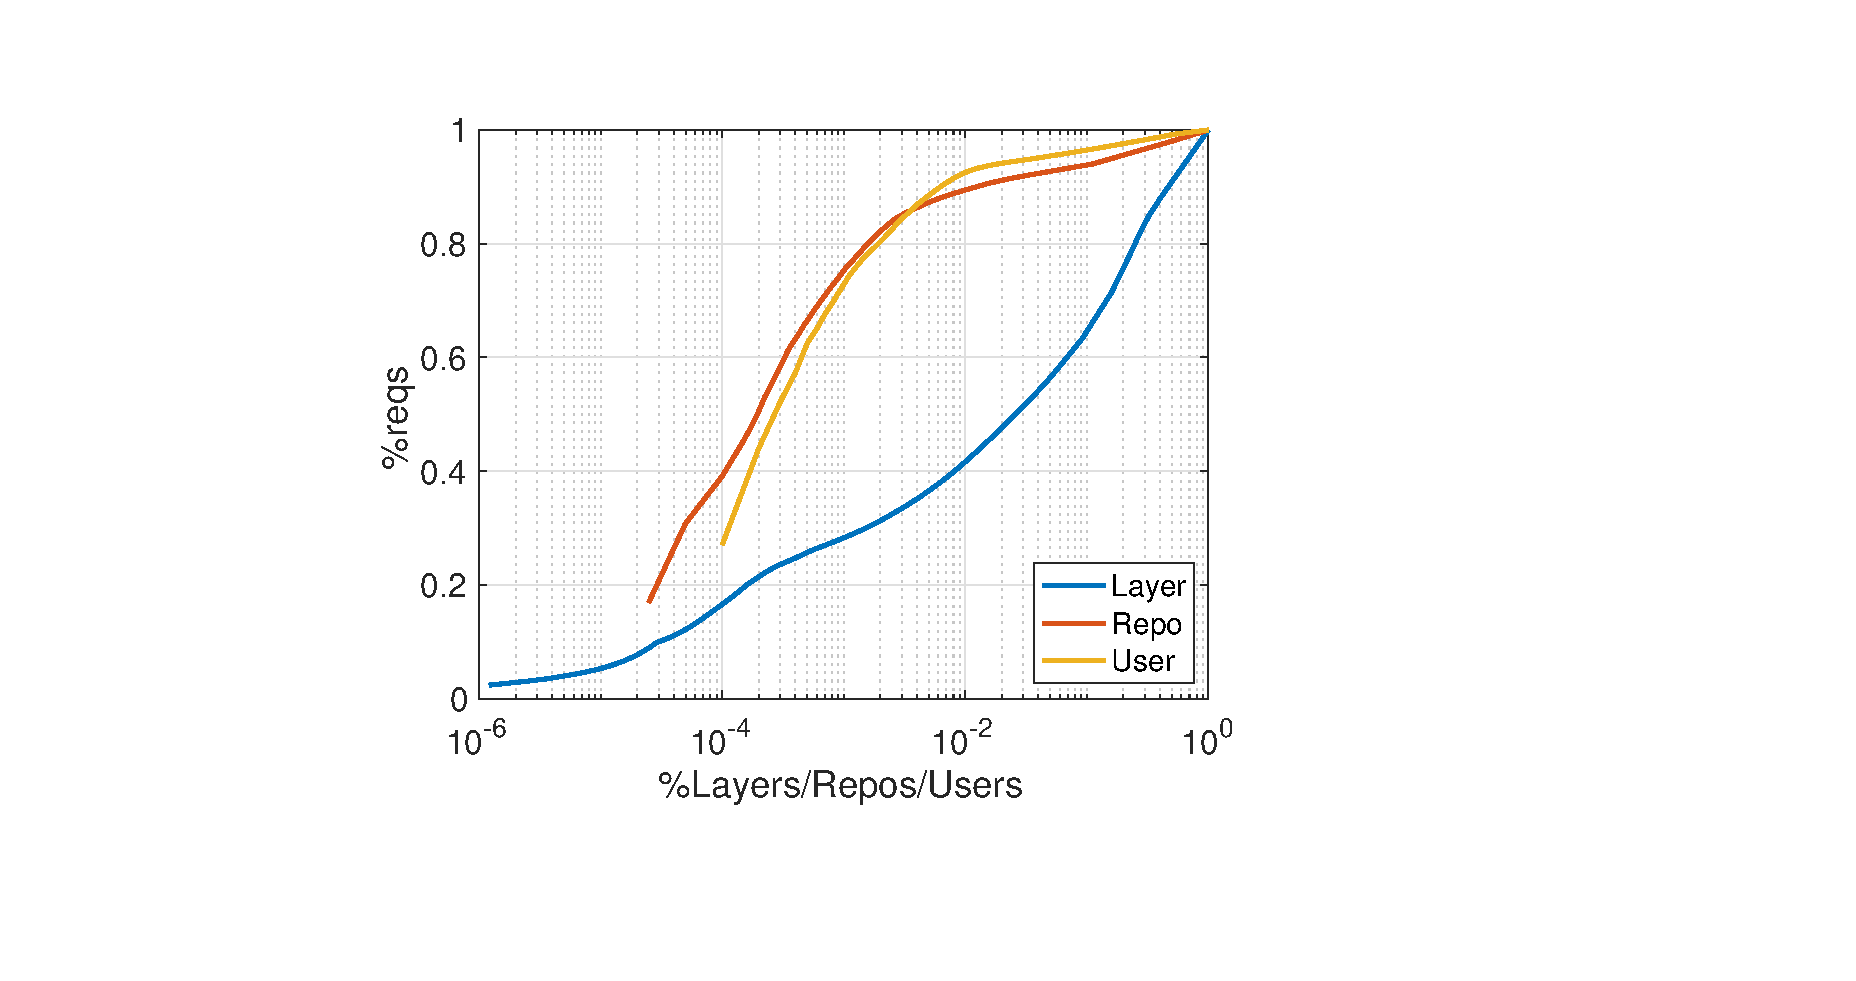
\includegraphics[width=1\textwidth]{graphs/skewness_cdf.eps}
			\caption{Popularity of layers, repos, and users.}
			\label{fig:sknewss}
		\end{minipage}
	\begin{minipage}{0.225\textwidth}
		\centering
		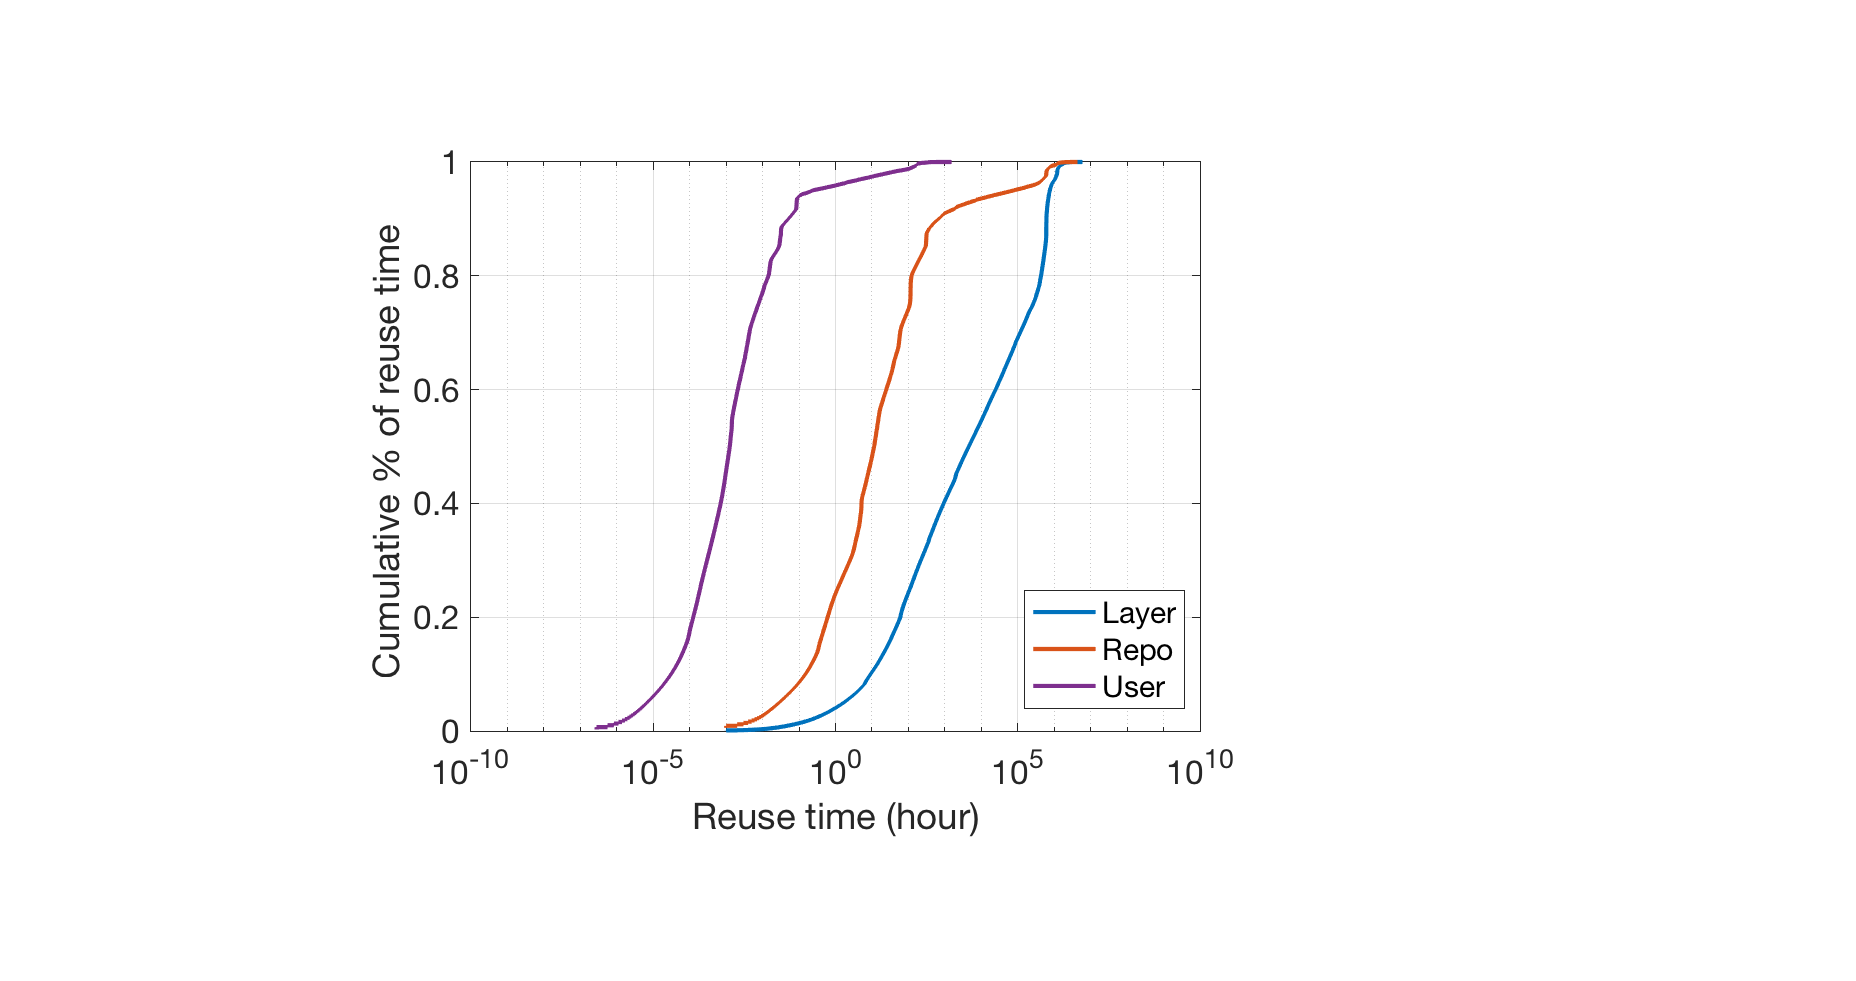
\includegraphics[width=1\textwidth]{graphs/reuse_time.eps}
		\caption{CDF of reuse time for layers, repos, and users.}
		\vspace{-3pt}
		\label{fig:reusetime}
	\end{minipage}
\end{figure}


\paragraph{Understanding layer access patterns.}
We analyzed the Dallas(\texttt{dal}) registry workload collected from IBM Container Registry over the course of 75 days~\cite{dockerworkload}. 
Figure~\ref{fig:sknewss} shows the registry accesses to layers and repositories, as well as users accesses to the \arb{layers??}. 
Layer accesses are heavily skewed. For example, 25\% of popular layers account for 80\% of all requests. 
For repository accesses and accesses by users, the skew is more significant than it is for layers. %10\% most frequently accessed repositories account for 94\% of all requests
94\% of all requests accessed only 10\% of the most frequently accessed repositories. Similarly, only 9\% of users, most active ones, issued 97\% of all requests. 
This means that only a few extremely active users create their repositories in the \texttt{dal} registry and issue the majority of requests to the registry.

Figure~\ref{fig:reusetime} shows the reuse time of layers and repositories, and reuse time by users.
Layer reuse time is the duration between two consecutive requests to the same layer or repository. Similarly,
reuse time by user is defined as duration between two consecutive requests issued by the same user. 
The layer reuse time is long.
The median reuse time of a layer is 1.3 hours. 80\% of repositories experience the highest request frequency, with a reuse time of $\~2$ minutes. 
90\% of users remain active for at least $0.06$ seconds.
%So for a registry, most of its stored layers are not accessed frequently given a very short time period while
%users can maintain active for a longer time. 
%This is because users can access multiple layers and manifests.
In other words, most of the layers stored in the
registry are not frequently requested in a very short
time period, while users remain active for a longer time.
This is because users can request different layers or manifests.

To quantify the efficacy of traditional LRU and pull-push prefetching,
we implemented an LRU algorithm and pull-push prefetching 
and replayed different number of requests from
IBM registry workload \texttt{dal} as shown in 
Figure~\ref{fig:lru_prefetching_hits}.
The hit ratio for LRU was found to be lower than $0.6$ 
while pull-push prefetching slightly improved the hit ratio to up to $0.8.$
\arb{say something whether this is good or bad... or is very low and show that LRU is not an effective mechanism for managing the proposed caches}

